



\section{PLENA Hardware System}

The overall configuration of PLENA is shown in \Cref{fig:PLENA_arch}. It employs instruction-level pipelining and mainly consists of three compute units: the Matrix Unit, the Vector Unit, and the Scalar Unit. All units are highly configurable, supporting multiple data types and precisions (\Cref{tab:design_space}), enabling the application of different quantization methods to the accelerator.

PLENA also includes two main on-chip SRAM blocks. The Vector SRAM acts as a scratchpad for computation, storing frequently used data such as activations, which do not need to be written back to HBM, thereby reducing memory access overhead. The custom Matrix SRAM is dedicated to loading weights and KV tensors and supports reading data in either transposed or untransposed access patterns with minimal extra resource cost and access overhead. 

\subsection{Asymmetric Arithmetic Data Path}
\label{sec:asymmetric}


To support asymmetric quantization strategies, PLENA natively supports multiple numeric formats---covering different data types and precisions---across its compute and memory units. This innovative \emph{asymmetric} data-handling configuration has the following characteristics.

(i)~Activations are stored in a high-precision floating-point (FP) format on-chip in the Vector SRAM, as they are more sensitive to quantization errors than KV or weights. (ii)~KV and weights, being less accuracy-sensitive, can be more aggressively quantized and staged in the Matrix SRAM using lower-precision MX formats (MXFP or MXINT). (iii)~An optional on-chip rotation step can suppress outliers before quantization to preserve accuracy.


Furthermore, when appending new \(K\) and \(V\) vectors to the KV cache in HBM during attention, we selectively apply a Hadamard-based rotation (algorithm detailed in \Cref{subsec:act_quant}) to suppress outliers before quantizing them to the MX data type and storing them in HBM. Since \(K\) and \(V\) are consumed exclusively by the attention GEMMs, they are loaded directly into the Matrix SRAM, where the inverse Hadamard transform is applied before use. These rotation/de-rotation stages can be selectively applied per tensor; for example, weights loaded into the matrix unit bypass the inverse transform.



\subsection{Flattened Systolic Array}

As shown in \Cref{fig:sa_compare_analysis}, long-context workloads frequently involve \textit{fat GEMMs} during the feed-forward (FFN) computation, where the batch-related dimension (typically $M$ in $(M,K)\times(K,N)$) is much smaller than the others, resulting in uneven matrix shapes (\Cref{fig:SA_Processing Flow}), while the reduction dimensions \(K\) tend to be very long, for example, the weight--activation GEMM reduces over the model’s hidden size (e.g., \(4{,}096\) for \llamaIIISmall and \(8{,}192\) for \llamaIIIBig). 

Additionally, in the FlashAttention stage, per-head \textit{fat GEMMs} operations are required. The head dimension is typically small (e.g., 128 for \llamaIIIBig), and the Grouped Query Attention (GQA) paradigm requires each key head to be multiplied by multiple query heads simultaneously. This results in low utilization of large-scale systolic arrays when performing per-head GEMMs in FlashAttention, as the computation dimension becomes relatively small.

\begin{figure}[!t]
  \centering
  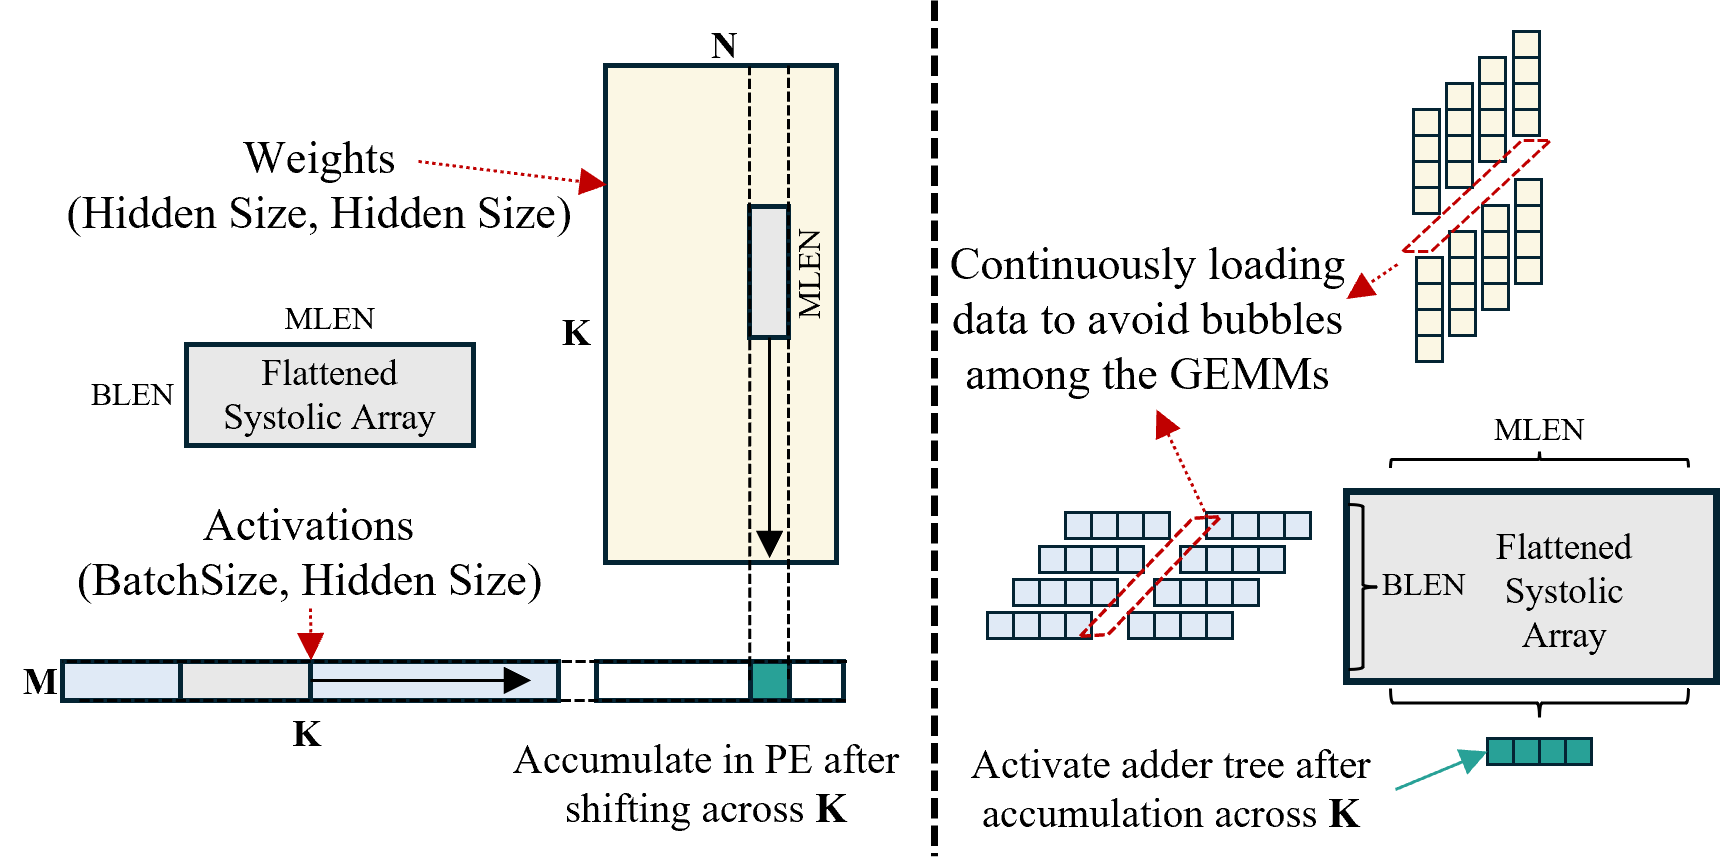
\includegraphics[width=0.48\textwidth]{Figures/Processing_flow.png}
  \caption{Processing flow for the weight--activation output stationary GEMM. Because memory capacity constrains batch size, the \(M\) dimension remains small. Setting \(\texttt{BLEN}=M\) on the flattened systolic array yields high utilization.}
  \label{fig:SA_Processing Flow}
  \vspace{-10pt}
\end{figure}


To improve hardware efficiency in the two most computationally intensive layers, we propose the \textit{flattened systolic arrays} architecture, which achieves a significantly higher utilization for both layers. For the FFN layer, each processing unit performs a \((\texttt{BLEN}, \texttt{MLEN}) \times (\texttt{MLEN}, \texttt{BLEN})\) GEMM, producing an output of shape \((\texttt{BLEN}, \texttt{BLEN})\). Typically, \(\texttt{BLEN}\) is configured to be much smaller than \(\texttt{MLEN}\) to match the workload characteristics of long-context LLM inference. For the FlashAttention module, the systolic array is partitioned into multiple smaller flattened array cores to support per-head GEMM computations, where each core performs a \((\texttt{BLEN}, \texttt{HLEN}) \times (\texttt{HLEN}, \texttt{BLEN})\) GEMM across \((\texttt{MLEN} // \texttt{HLEN})\) heads in parallel.

This flattened systolic array is designed for the output-stationary dataflow in order to maintain a high utilization. As shown in \Cref{fig:SA_Processing Flow}, operands stream along the large reduction dimension \(K\) while partial sums remain stationary in the PEs. The array is then fully pipelined, eliminating idling bubbles between consecutive GEMM tiles.
The microarchitecture of the flattened systolic array is shown in \Cref{fig:Flattened_Systolic_Array}. It is built from a series of small square-shaped systolic arrays (\emph{sub-arrs}), each consisting of a grid of processing elements (PEs). Each PE repeatedly performs multiply–accumulate operations and passes data to its neighboring PEs below and to the right across the array. As described in \Cref{sec:asymmetric}, the systolic array is designed to natively accept data in the MX format.


\begin{figure}[t]
  \centering
  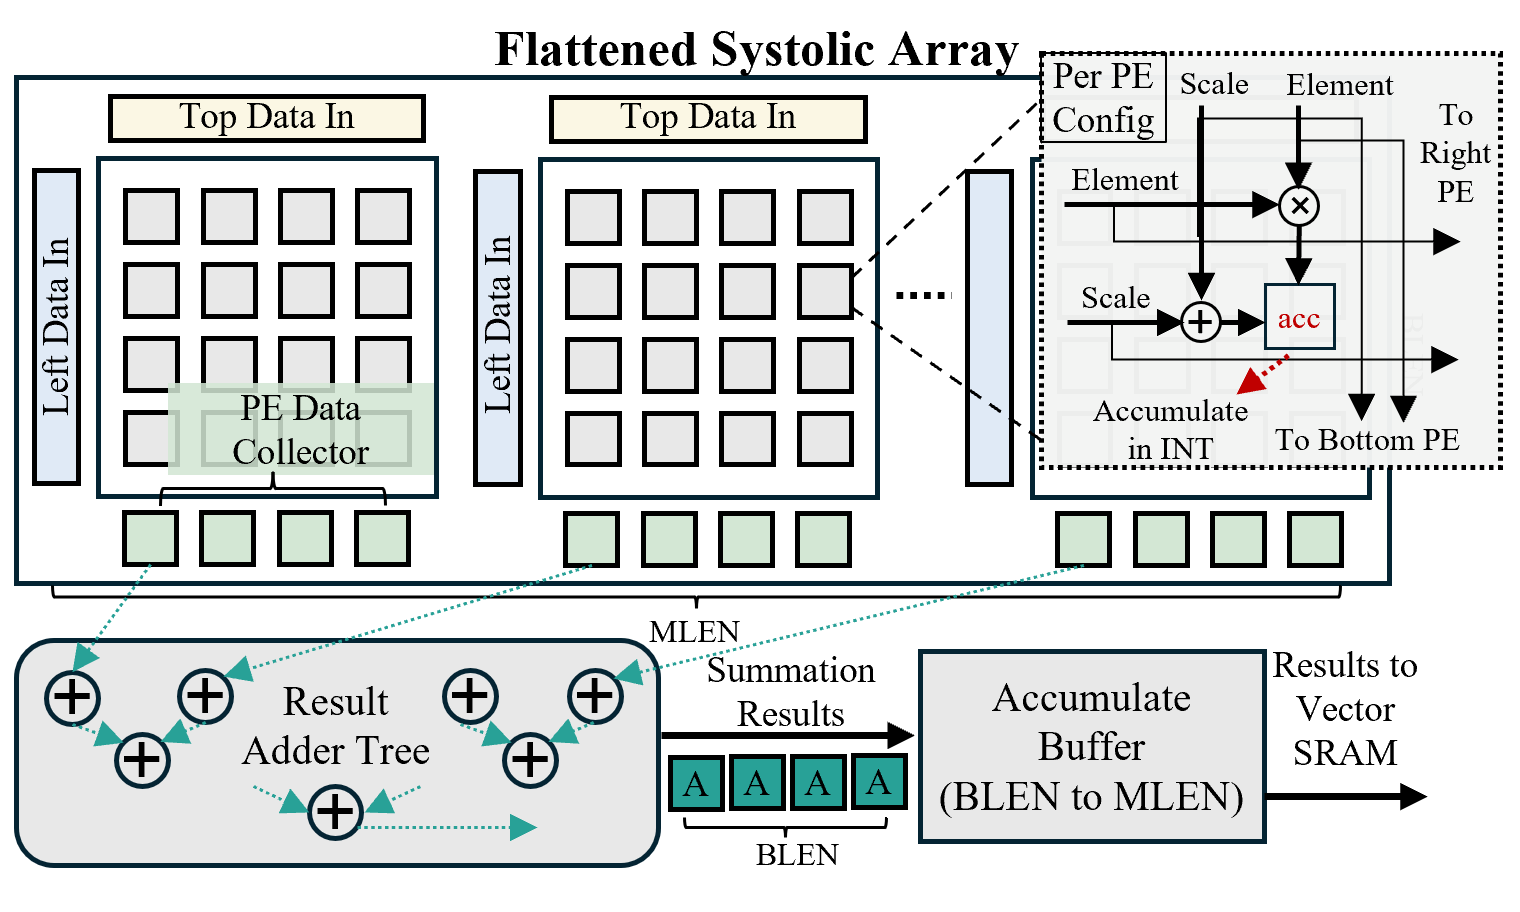
\includegraphics[width=0.48\textwidth]{Figures/Flattened_Sys.png}
    \caption{
    At each cycle, the flattened systolic array fetches two \texttt{MLEN}-wide inputs: one from the Matrix SRAM (top) and one from the Vector SRAM (left). The inputs are buffered and reordered, then partitioned into \(\texttt{MLEN}/\texttt{BLEN}\) subvectors (assuming \texttt{MLEN} is divisible by \texttt{BLEN}), each of width \texttt{BLEN}. Each subvector is forwarded to a corresponding sub-array from the top and left directions. 
    The scales and elements are streamed separately to each subarray. For improved resource efficiency, each PE consumes MX-format inputs and performs accumulation in INT precision. The accumulated results are converted to the target activation precision before being written back to the Vector SRAM.
    }
  \label{fig:Flattened_Systolic_Array}
  \vspace{-15pt}
\end{figure}


However, a matrix unit composed solely of \emph{sub-arrs} is insufficient to complete a $(\texttt{BLEN}, \texttt{MLEN})\times(\texttt{MLEN}, \texttt{BLEN})$ GEMM. Each array accumulates only partial sums for a fragment of the result; producing a complete \((\texttt{BLEN}, \texttt{BLEN})\) output requires a cross-array reduction that sums the partial sums held in the PEs across the tiled row. To address this, we integrate a result adder tree (see \Cref{fig:Flattened_Systolic_Array}) that performs the cross-array summation efficiently. This unit is invoked via a dedicated instruction M\_SUM, as only one cross-array summation is required when computing GEMM along the large reduction dimension. This prevents bubbles and improves computational efficiency.


\subsection{Asymmetric Memory Balancing}
Our memory system is characterized by two key properties: 1) Support for asymmetric precisions, variable-length memory transfers, and strided loads/stores to HBM; and 2) Latency hiding for HBM accesses via an memory load unit that operates in parallel with the main execution, enabling high bandwidth utilization.

To make more effective use of HBM capacity, as discussed in \Cref{sec:asymmetric}, all data stored in HBM is kept in the MX format. Since concatenating each data block with its per-block scale would rarely yield a combined size that aligns with a power-of-two memory boundary, we instead store the blocks and their corresponding scales for each tensor separately to ensure that both are properly aligned with the memory boundary. This layout improves memory efficiency while maintaining data locality, as illustrated in \Cref{fig:HBM_sys}.



\begin{figure}[!t]
  \centering
  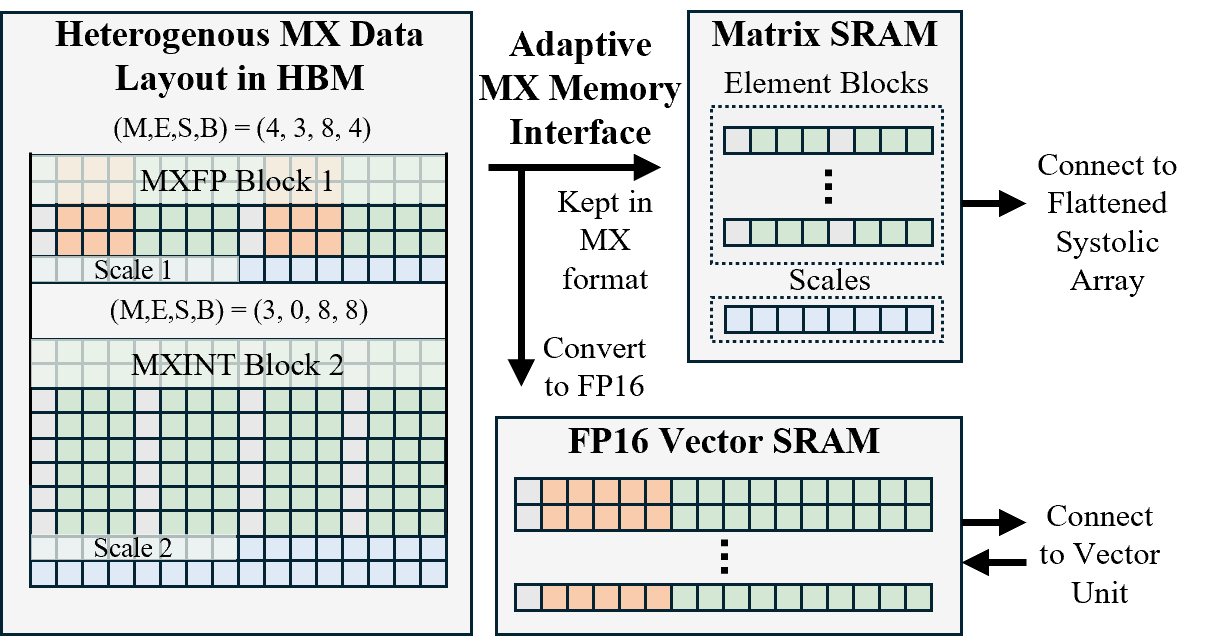
\includegraphics[width=0.48\textwidth]{Figures/HBM_sys.png}
  \caption{Data layouts and data paths for the memory system. Data with different MX precisions and datatypes are stored following a unified HBM storage pattern. A conversion to FP16 is performed as the data enter the Vector SRAM, which serves as the scratchpad for the vector unit; the vector unit operates in high-precision FP16. For the Matrix SRAM, MX-formatted data loaded from HBM can be stored directly without additional conversion.}
  \label{fig:HBM_sys}
  \vspace{-5pt}
\end{figure}


The memory load unit is critical for fully utilizing HBM bandwidth. Hardware prefetch engines are integrated into both the Matrix and Vector SRAMs, enabling background fetching from HBM and streaming data into each SRAM while the rest of PLENA continues executing other instructions. This sustains full utilization of the matrix unit and avoids stalls due to HBM latency. The two load units are controlled directly by dedicated instructions, H\_LOAD\_M for the Matrix SRAM and H\_LOAD\_V for the Vector SRAM. The load size for each instruction is configurable and specified through the \texttt{M\_Load} and \texttt{V\_Load} parameters.

\subsection{PLENA ISA}

Our customized ISA is designed to cover all operations required for transformer inference. The instructions are structured to balance efficiency with flexibility and are built to support multiple transformer-based models and computation optimizations. In addition to FlashAttention, the ISA also supports different transformer variants, such as MHA, MLA~\cite{MLA}, and MoE~\cite{MoE}. A brief summary is provided in Table~\ref{tab:Custom_ISA}.

\begin{table}[t]
\centering
\setlength{\tabcolsep}{6pt}
\renewcommand{\arraystretch}{1.3}
\caption{An overview of the PLENA ISA.}
\begin{tabular}{
    >{\centering\arraybackslash}m{1.3cm}
    m{5cm}
    >{\centering\arraybackslash}m{1.3cm}
}
\toprule
\textbf{Types} & \textbf{Descriptions} & \textbf{\# Instr.} \\
\midrule
Matrix(M)  & Controls GEMM and GEMV operations, with or without matrix transposition & 6 \\
Vector(V) & Performs elementwise and reduction operations, and rotation for quantization & 13 \\
Scalar(S) & Performs scalar INT and FP arithmetic & 17 \\
HBM(H) & Handles data transfers between HBM and the Matrix/Vector SRAMs & 3 \\
Control(C) & Defines operation settings such as the HBM address, nested-loop configuration, and other execution parameters & 8 \\
\bottomrule
\end{tabular}
\label{tab:Custom_ISA}
\end{table}


\begin{figure}[t]
  \centering
  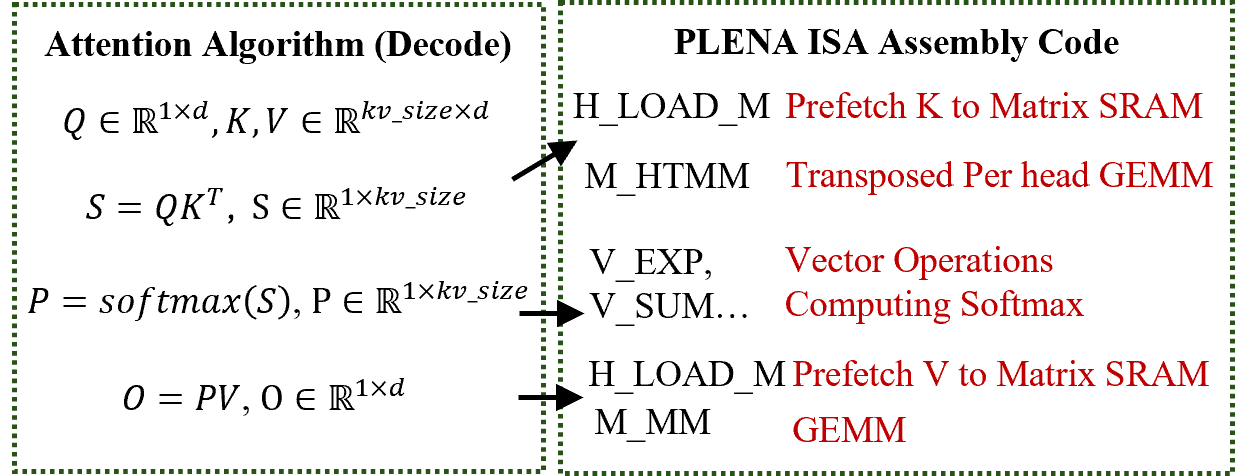
\includegraphics[width=0.48\textwidth]{Figures/custom_isa.png}
  \caption{Example of how the single batch single head attention algorithm maps onto PLENA’s custom ISA. Instruction prefixes denote the unit type (e.g., M\_ for Matrix instructions).}
  \label{fig:custom_isa_example}
\end{figure}

To achieve the efficiency and flexibility balance, the ISA is designed to minimize overhead while maximizing utilization of compute and memory resources. This is achieved through features such as tile-level scheduling, which enables fine-grained control of computation and memory instructions at the tile granularity. Furthermore, the ISA defines dedicated instruction classes (Matrix, Vector, Scalar, Memory, and Control) that decouple responsibilities, simplify scheduling, and allow flexible mixing across different computation types.  

Instructions (32 bits each) are dynamically dispatched from the CPU to the instruction buffer via PCIe. In addition to computation, matrix and vector instructions also control read and write operations to their respective SRAMs. Address manipulation is handled by scalar instructions.


\vspace{-2pt}
\subsection{Matrix SRAM}
\label{sec:matrix_sram}

The matrix SRAM is designed to support both transposed and non-transposed accesses without additional latency or data movement overhead. This design specifically targets optimizing the transposed matrix multiplication (\(QK^{\top}\)) in FlashAttention (see \Cref{fig:custom_isa_example}) with low hardware overhead.

In autoregressive inference, explicitly transposing large tiles during the $(QK^{\top})$ computation introduces significant area, energy, and latency overhead. Storing $(K^{\top})$ directly in HBM is also impractical, as newly generated $K$ vectors must be appended to the KV cache during decoding. Consequently, transposition must be performed on the fly, motivating an SRAM organization that supports both row and column access efficiently without explicit data rearrangement.

As shown in \Cref{fig:Transpsoed_SRAM}, the matrix SRAM distributes each logical row across multiple sub-SRAM banks, storing elements of the same row in different banks at distinct addresses. This layout ensures that row and column accesses map to separate banks, allowing transposed and non-transposed accesses to proceed in parallel without bank conflicts, thereby preserving bandwidth and avoiding explicit data movement.




\begin{figure}[!t]
  \centering
  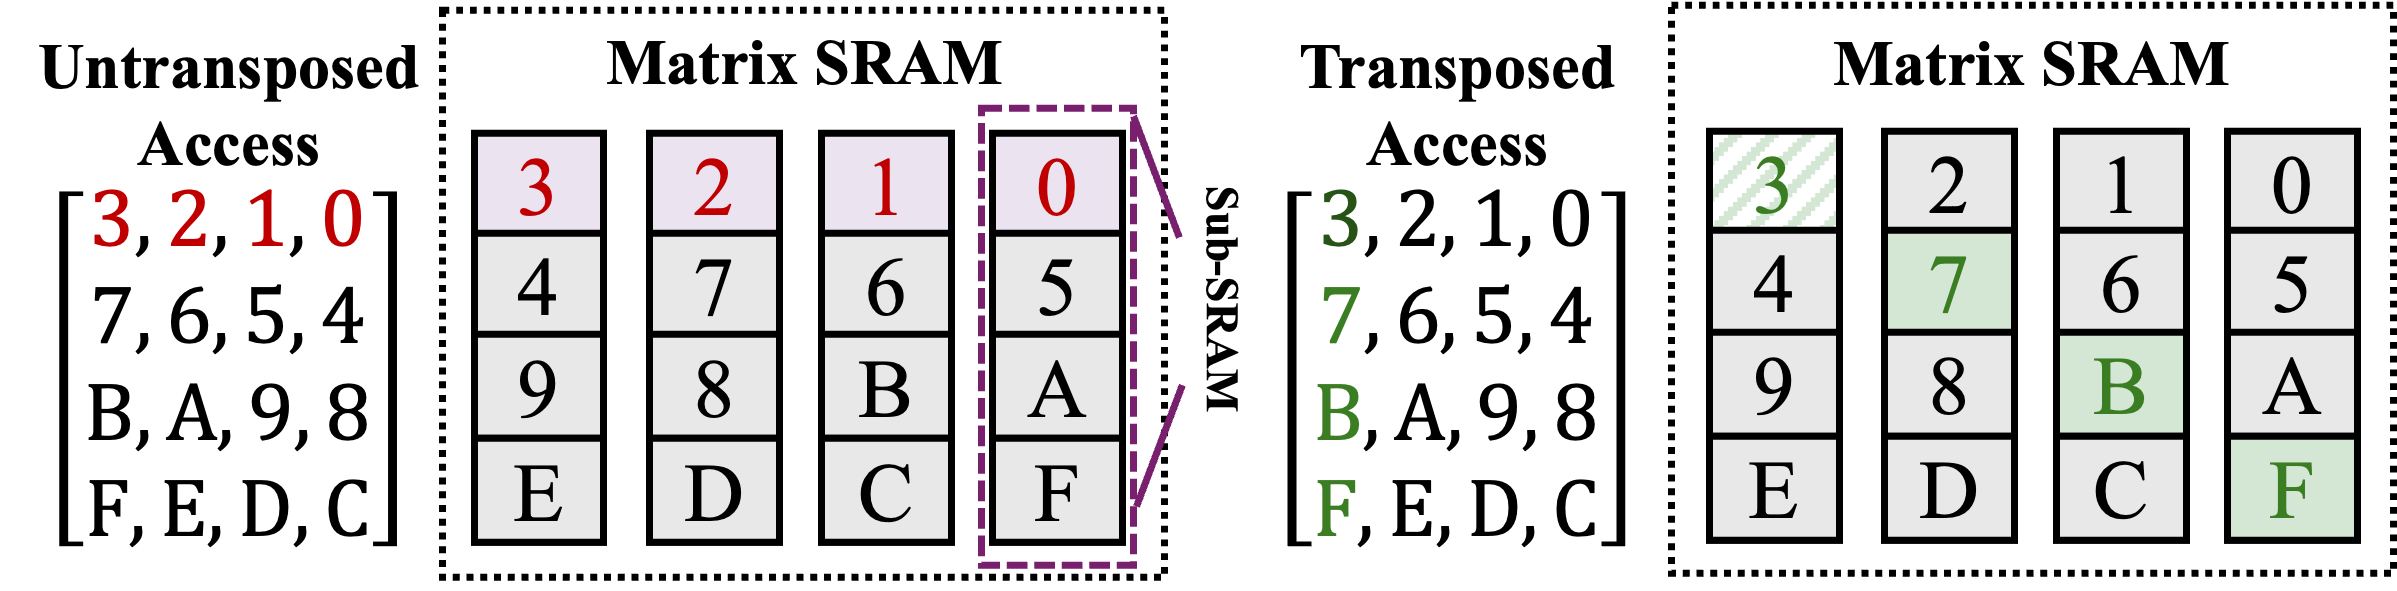
\includegraphics[width=0.47\textwidth]{Figures/Transposed_SRAM.png}
    \caption{The transposable matrix SRAM design ensures that, for both untransposed and transposed accesses, each sub-SRAM is accessed by at most one element per cycle. As a result, no additional access cycles are introduced.}
  \label{fig:Transpsoed_SRAM}
  \vspace{-10pt}
\end{figure}



\subsection{Supporting FlashAttention}
\label{subsec:flashatten}
Most existing systolic-array–based accelerators do not natively support FlashAttention due to these three key elements: 
\begin{enumerate}
    \item They do not support tile-level overlapping of off-chip memory prefetching with computation, resulting in additional latency overhead as execution must wait for data to be loaded from off-chip memory.
    \item They lack memory-layout support such as transpose-on-read and efficient strided/blocked streaming.
    \item They expose only GEMM primitives and lack in-line, row-wise reductions and nonlinear operations (\texttt{max/sum}, \texttt{exp}, \texttt{div}) required for the online softmax.
    \item Their ISAs enforce fixed scheduling and coarse-grained kernel boundaries, which restrict fine-grained tile-by-tile execution and prevent the fused computation pattern.
\end{enumerate}

In PLENA, we address (1) and (2) through the proposed \emph{Matrix SRAM} (see \Cref{sec:matrix_sram}), which enables instruction-level control of memory prefetching and supports transpose-on-read with low overhead. Challenge (3) is addressed by vector and scalar units that implement reductions and element-wise operations. The vector width (\texttt{VLEN}) is configurable to match the tile dimensions used by FlashAttention. The computation precision is also configurable, but is typically set to higher precision (e.g., FP12) to preserve numerical accuracy during the softmax computation. For (4), our custom ISA provides composable, fine-grained control, enabling persistent, tile-by-tile scheduling of the fused attention pipeline. This allows each stage of FlashAttention to be orchestrated individually at tile granularity. Together, these mechanisms enable PLENA to support FlashAttention natively and efficiently.

\begin{figure}[!t]
  \centering
  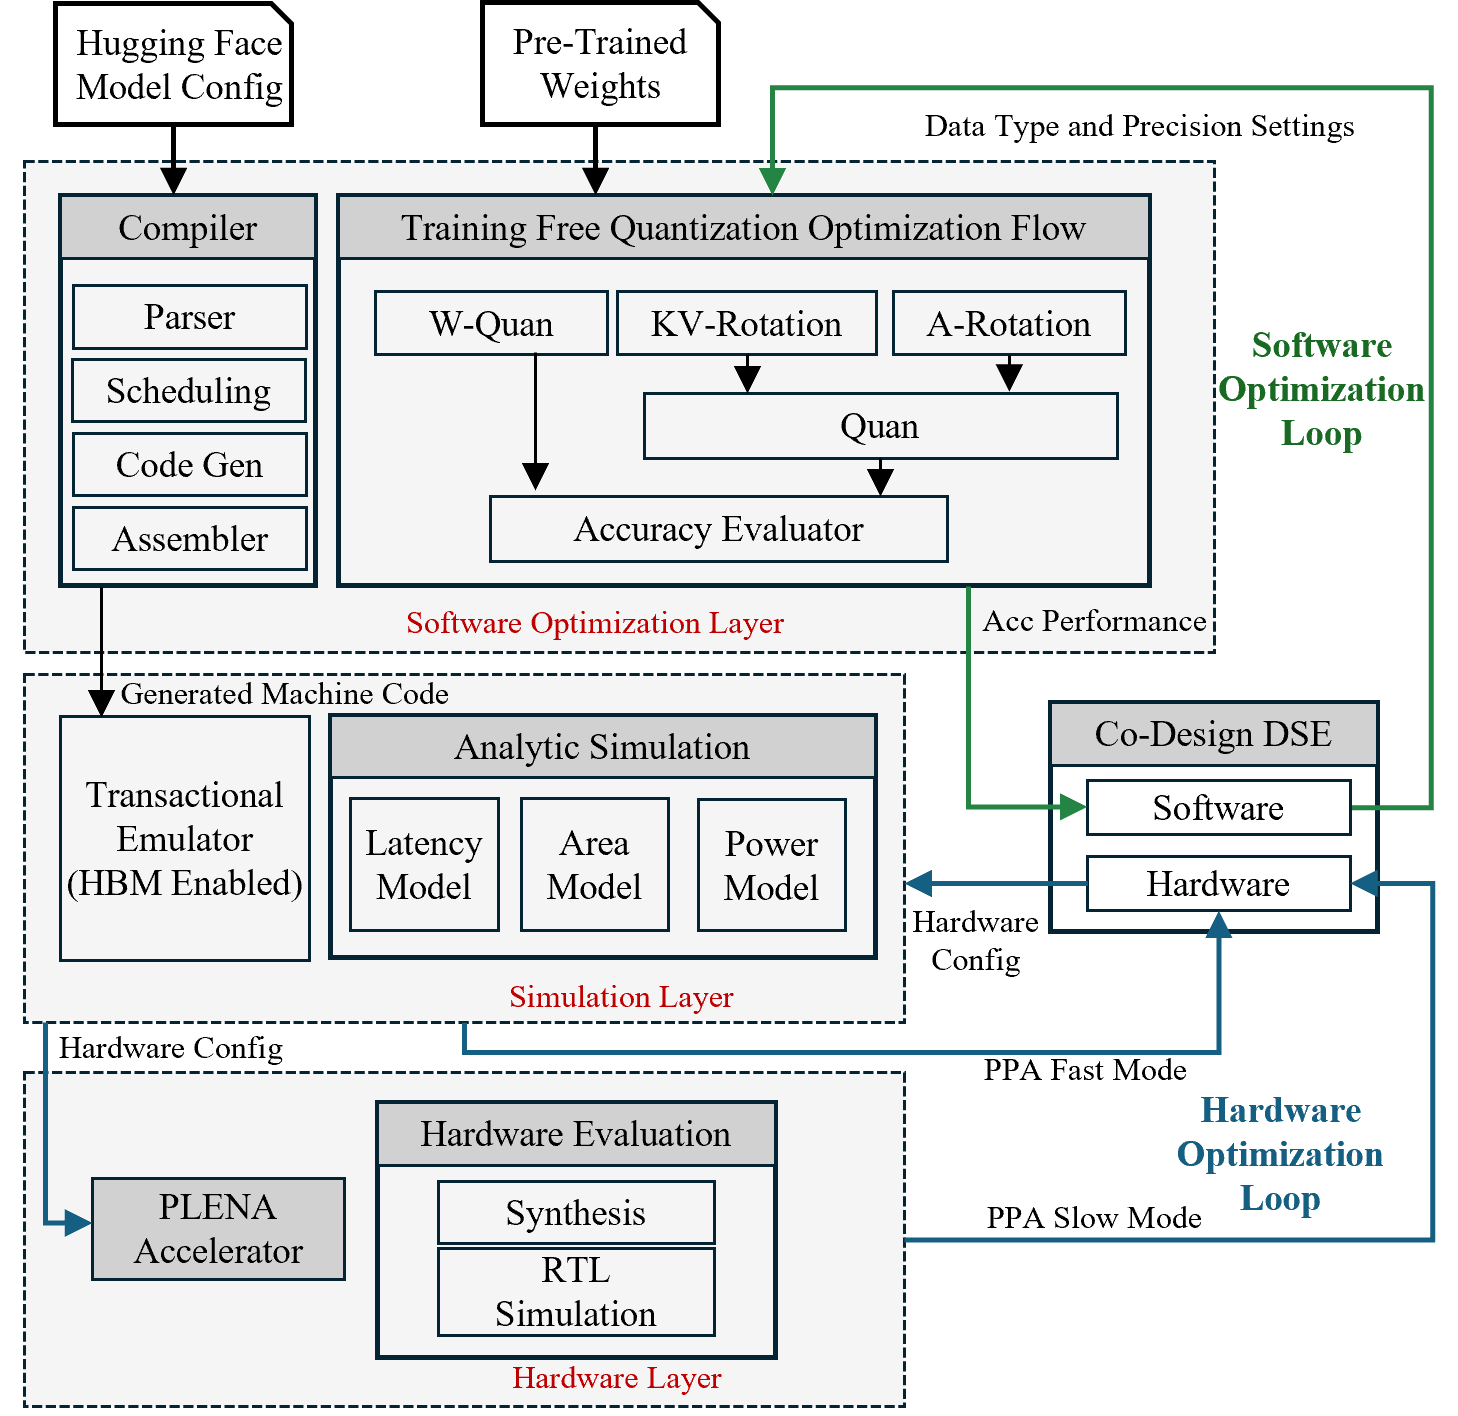
\includegraphics[width=0.47\textwidth]{Figures/Design_Flow.png}
    \caption{The co-design framework consists of hierarchical layers (actual hardware, transactional emulator, and analytic simulator) with different fidelities. The transaction-level simulator offers good fidelity (cycle-accurate) while achieving an over $200\times$ speedup compared to RTL simulation, and is used for our Co-Design DSE.}
  \label{fig:PLENA_overview}
  \vspace{-10pt}
\end{figure}



\subsection{The PLENA Compilation and Simulation Stack}

PLENA provides a comprehensive design and evaluation framework that can rapidly adapt to new models or new hardware accelerators and optimize for them (\Cref{fig:PLENA_overview}).


Since Transformer computations are highly repetitive and structurally uniform, the PLENA compiler is intentionally kept lightweight: it parses configuration metadata from the model configuration file and maps it onto a predefined PLENA custom ISA assembly template.

To evaluate architectural trade-offs, we developed a transaction-level (cycle-approximate) emulator in Rust that executes the generated machine code in an event-driven manner. The emulator models compute execution, instruction scheduling, and memory transactions at cycle granularity. It is integrated with Ramulator~\cite{Ramulator} and DRAMSys~\cite{dramsys} to provide detailed off-chip memory timing and bandwidth modeling, including bank-level behavior. This enables quantitative analysis of memory–compute interaction, which is critical because memory bandwidth constitutes a primary bottleneck in long-context LLM inference.

The emulator supports the full PLENA architectural design space, including asymmetric mixed-precision arithmetic (\Cref{sec:asymmetric}). By bridging analytic modeling and RTL simulation, it enables accurate evaluation of architectural mechanisms—such as flattened systolic mapping and on-chip FlashAttention, while remaining significantly faster than RTL simulation. We plan to open-source this emulator to facilitate research on LLM accelerator architectures.


\begin{table}[!t]
\centering
\setlength{\tabcolsep}{3pt}
\renewcommand{\arraystretch}{1.15}
\caption{Average error rates across five trials for different simulation levels, compared with RTL and synthesis results for a single Transformer block of the \llamaIIIBig model.}
\begin{tabular}{lcccc}
\toprule
\textbf{Evaluator / Model} & \textbf{Latency} & \textbf{Area} & \textbf{Power} & \textbf{Exe Time} \\
\cmidrule(lr){1-5}
Analytic Simulator       & 11.32\% & 4.79\% & 23.81\% & 8ms \\
Transaction Emulator     & 4.17\% & not supp & not supp & 4.3mins\\
RTL Sim. / Synth.    & ref & ref & ref & 14hrs\\
\bottomrule
\end{tabular}
\label{tab:eval_models}
\vspace{-5pt}
\end{table}


We validated the simulator against our full RTL implementation: it closely matches the RTL synthesis results in both execution latency and numerical accuracy while delivering roughly a $200\times$ speedup, as shown in \Cref{tab:eval_models}.



